\documentclass[border=1mm]{standalone}
%\documentclass[11pt]{article}
\usepackage{amsfonts,tikz,tikz-layers}
\usetikzlibrary{fadings,quotes, shapes,calc,decorations.markings}
\usetikzlibrary{patterns}
\usetikzlibrary{shadows.blur}
\usetikzlibrary{shapes,shapes.geometric,positioning, arrows, arrows.meta}
\usetikzlibrary{backgrounds}
\begin{document}
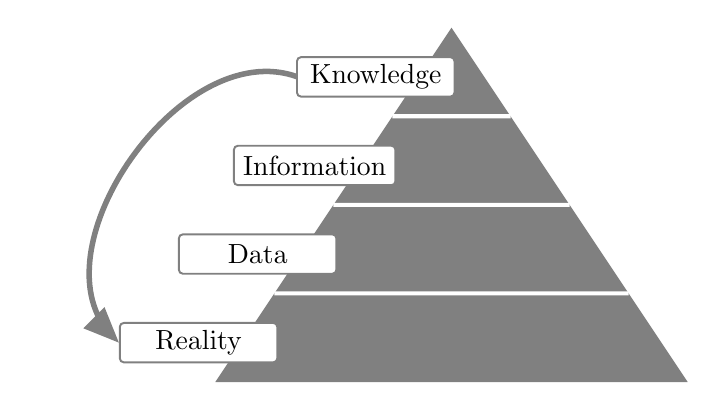
\begin{tikzpicture}[line width=.7pt]
% Triangle
\fill[gray] (0,0)--(6,0)-- coordinate[pos=.25] (p1) coordinate[pos=.5] (p2) coordinate[pos=.75] (p3) (3,4.5)-- coordinate[pos=.25] (n3) coordinate[pos=.5] (n2) coordinate[pos=.75] (n1) coordinate[pos=1] (n0) cycle;
\draw[white,line width=1.5pt] (n1)--(p1);
\draw[white,line width=1.5pt] (n2)--(p2);
\draw[white,line width=1.5pt] (n3)--(p3);
% Text boxes
\node[draw=gray, minimum width=2cm,minimum height=.5cm, fill=white, shift={(.8,.5)}, rounded corners=.5mm, text=black, anchor=east,inner ysep=0pt] (kn) at (n3) {Knowledge};

\node[draw=gray, minimum width=2cm,minimum height=.5cm, fill=white, shift={(.8,.5)}, rounded corners=.5mm, text=black, anchor=east, inner ysep=0pt]  at (n2) {Information};

\node[draw=gray, minimum width=2cm,minimum height=.5cm, fill=white, shift={(.8,.5)}, rounded corners=.5mm, text=black, anchor=east, inner ysep=0pt] at (n1) {Data};

\node[draw=gray, minimum width=2cm,minimum height=.5cm, fill=white, shift={(.8,.5)}, rounded corners=.5mm, text=black, anchor=east, inner ysep=0pt] (re) at (n0) {Reality};
% Curved arrow
\begin{scope}[on behind layer]
\draw[gray, -triangle 45, line width=2pt] ([xshift=.2mm]kn.west) to [out=160, in=90+45, looseness=1] (re.west);
\end{scope}
\end{tikzpicture}
\end{document}
